\section{Experiments Results}
\label{sec:expr}
%\subsection{Quality Evaluation Metrics}
%
We used two metrics for evaluating the results of the proposed approaches, one of these metrics is used by SeeDB to evaluate the quality of aggregate views \cite{DBLP:journals/pvldb/VartakMPP14}. Through the next set of experiments, we evaluate the impact of our proposed optimizations techniques.
%

\noindent\textbf{Metrics:} To evaluate the quality and correctness of the proposed algorithms, we used the following metrics:
%\[
%\text{Relative Error} (RelErr) = \frac{1}{k} \sum^{k}_{i=1}{ \frac{| U'(v_i) - U(v_i) |}{U(v_i)} }
%\]
%
%Where, $U'(v_i)$ is the utility of $i$-th view outputted by our proposed methods, $U(v_i)$ is the utility of the $i$-th view outputted by SeeDB baseline, and $k$ is the number of top interesting views.
%

%\noindent\textbf{SeeDB Metrics:} SeeDB evaluates the performance of its pruning optimizations along two dimensions: latency and quality of results \cite{vartakseedb}. 
%
%It measures the quality of results in two ways:
\begin{itemize}
\item Accuracy: if $\{VS\}$ is the set of aggregate views with the highest utility, and $\{VT\}$ is the 
set of aggregate views returned by SeeDB baseline, then the accuracy is defined as:
%\[
%Accuracy = \frac{1}{|VT|} * | VT \bigcap VS| 
%\]
\[
Accuracy = \frac{1}{|VT|} * \sum{x}  \text{   where  }  \begin{cases}   x = 1 & \text{ if } VT_i = VS_i \\ x = 0 & otherwise \end{cases}
\]
i.e., accuracy is the fraction of true positions in the aggregate views returned by SeeDB.
%\mas{as I mentioned MANY times now, there is no positions in that equation!!}
%
\item distance-error: since multiple aggregate views can have similar utility values, we use utility distance as a measure of how far SeeDB results are from the true top-k aggregate views. 
%
Formally, SeeDB \cite{vartakseedb} defines distance error as the difference between the average utility of $\{VT\}$ and the average utility of $\{VS\}$:
\[
\text{distance-error} = \frac{1}{k} (\sum_{i}{ U(VT_i)} - \sum_{i}{U(VS_i)})
\]
%
\end{itemize}
%
\subsection{ Quality Evaluation Across Aggregate Functions }
In these experiments we evaluate quality of the recommended visualizations produced by proposed techniques 
 across different aggregate functions namely: \emph{Count, Sum, Average, Min, and Max}. 
The dataset used is $Flight$ database for flight delays in year 2008 obtained from 
The U.S. Department of Transportation's Bureau of Transportation Statistics (BTS) with 
size 250 K tuples \footnote { http://www.transtats.bts.gov/}. 
The dataset contains 10 dimension attributes and 10 measures attributes. 
We run this experiment to assess the quality of the recommended views 
over each aggregate function \emph{separately} 
 with a space size(SP)=$1 \times 10 \times 10=100$ possible views and 
the deviation metric is Earth Movers Distance (EMD). All Experiments were executed 
5 times and obtained the averaged results, we concerned with evaluating the 
the accuracy and utility of views produced by the proposed algorithms along 
limited number of views (referred as Views Limit) $R$ and various sets of top deviated views $K$. In experiments, the analyst
posed a query\\
 $Q:$ select * from ontime2008 where uniquecarrier ='American Airlines Inc.' \\ 
We implement two baseline strategies SeeDB baseline strategy processes the entire data 
and does not discard any views ($SeeDB baseline$). It thus provides an upper bound on 
latency and accuracy and lower bound on error distance.
The other baseline strategy we evaluate is the random strategy ($SeeDB_Rnd$) that 
returns a random set of k aggregate views as the result. This strategy gives a lower bound on 
accuracy and upper bound on error distance: for any technique to be useful, it must do 
significantly better than $SeeDB_Rnd$.

In the next experiments, we vary $R$ — the number of limited visualizations that explored denoted as \emph{Views Limit} 
to recommend $K=20$ visualizations and measure the accuracy, and error-distance for each of our
strategies along different aggregate functions.\\

In summary, $Sela$ and $DimsHisto$ algorithms both produce results with accuracy $>80\%$ and near-zero utility
distance for all aggregate functions and a variety of $R$ Views Limits particularly when Views Limits=60 views as shown in figures \ref{fig:SumA2},\ref{fig:AvgA2}, and \ref{fig:CountA2}. Moreover, they produce results with $100\%$ accuracy and zero distance error after that limit. $Sela$ does slightly better than $DimsHisto$ as $Sela$ evaluates the recommended views by capturing the change of the selectivity ratios of dimension attributes that create views in both result set and reference set however, $DimsHisto$ scores accuracy $100\%$ in figure \ref{fig:CountA2} for aggregate function \emph{Count} because the generated histograms from this algorithm are similar to the views created by counting dimension attribute values across different measure attributes. Algorithm $Diff_DVal$ is the lowest accuracy and the highest distance error among other algorithms specially for aggregate functions \emph{Max and Min} as shown in figures \ref{fig:MaxA2} and \ref{fig:MinA2} as it assess recommended views based on the difference of the distinct values only. 

\begin{figure}[h]
  \begin{subfigure}[b]{0.32\textwidth}
    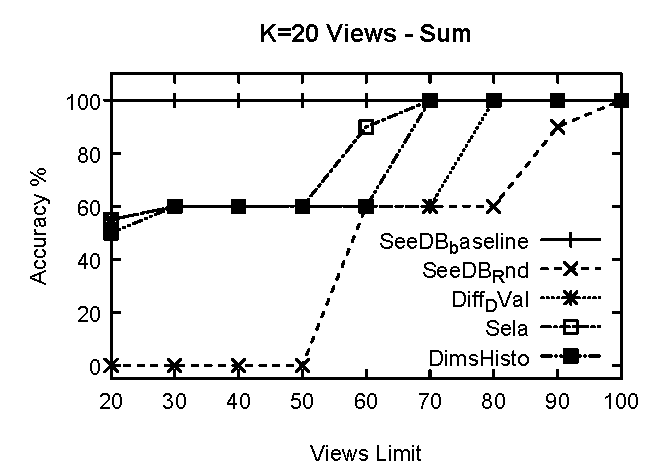
\includegraphics[width=\textwidth]{SumA2.pdf}
    \caption{Sum}
     \label{fig:SumA2}%
  \end{subfigure}
  %
  \begin{subfigure}[b]{0.32\textwidth}
    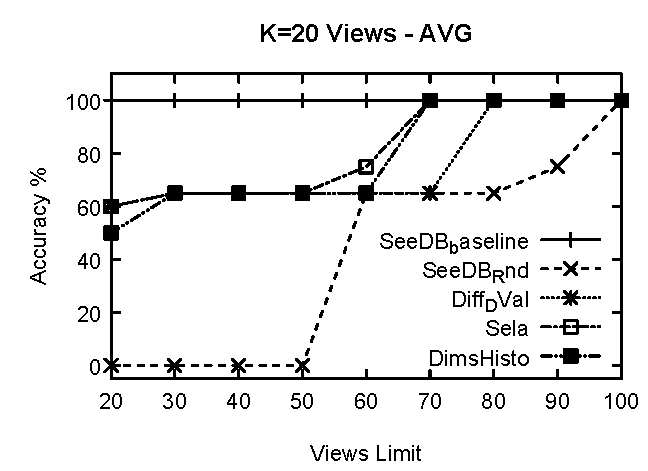
\includegraphics[width=\textwidth]{AvgA2.pdf}
     \caption{Average}
        \label{fig:AvgA2}
  \end{subfigure}
  \begin{subfigure}[b]{0.32\textwidth}
    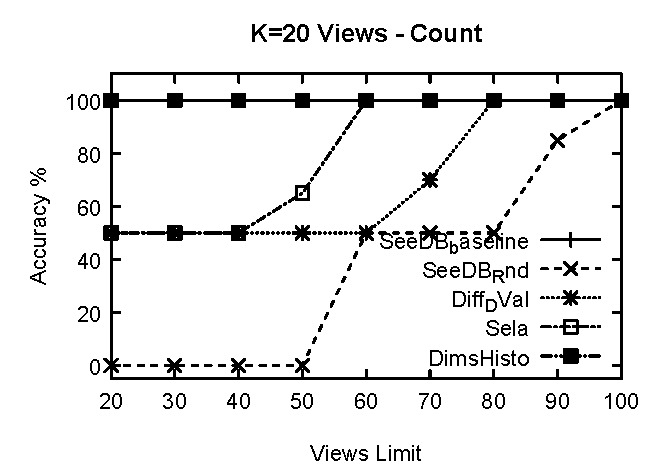
\includegraphics[width=\textwidth]{CountA2.pdf}
     \caption{count}
        \label{fig:CountA2}
  \end{subfigure}
  \caption{Accuracy on varying view space sizes for the Algorithms $Sela$ ,$Diff_DVal$, $DimsHisto$, and $SeeDB_Rnd$}
\end{figure}

\begin{figure}[h]
  \begin{subfigure}[b]{0.32\textwidth}
    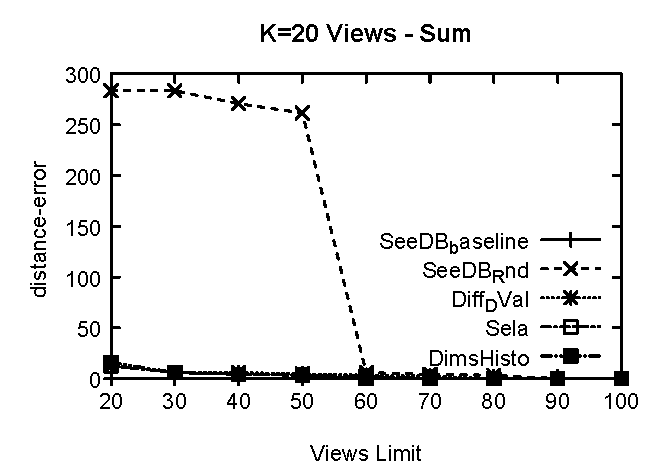
\includegraphics[width=\textwidth]{SumD2.pdf}
    \caption{Sum}
        \label{fig:SumD2}%
  \end{subfigure}
  %
  \begin{subfigure}[b]{0.32\textwidth}
    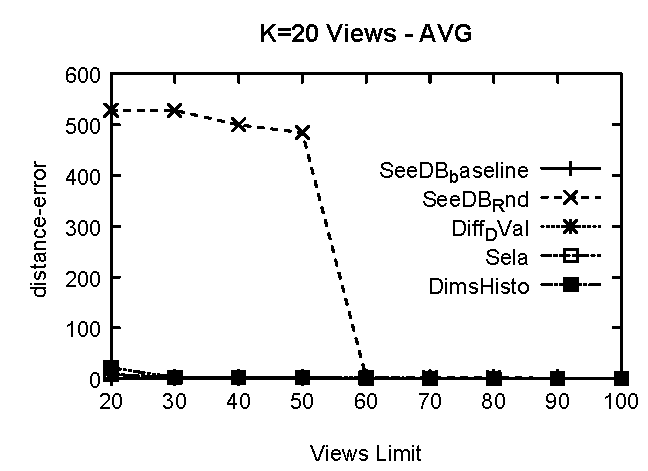
\includegraphics[width=\textwidth]{AvgD2.pdf}
     \caption{Average}
        \label{fig:AvgD2}
  \end{subfigure}
  \begin{subfigure}[b]{0.32\textwidth}
    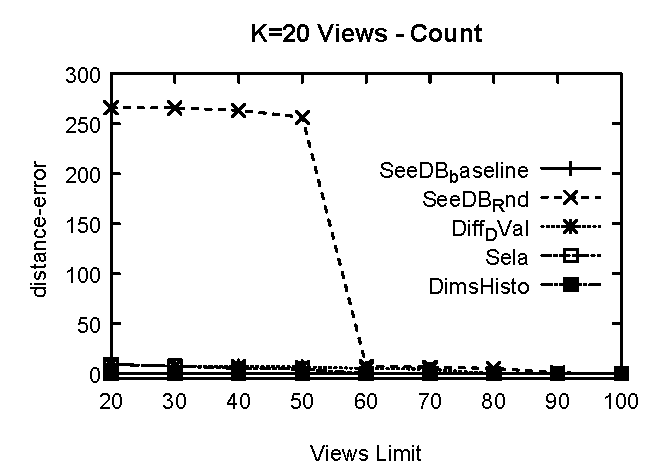
\includegraphics[width=\textwidth]{CountD2.pdf}
     \caption{count}
        \label{fig:CountD2}
  \end{subfigure}
  \caption{Distance-error on varying view space sizes for the Algorithms $Sela$ ,$Diff_DVal$, $DimsHisto$, and $SeeDB_Rnd$}
\end{figure}

As shown in figures \ref{fig:SumD2},\ref{fig:AvgD2},\ref{fig:CountD2} The proposed algorithms produce results near-zero distance-error for all aggregate functions compared with lower baseline strategy $SeeDB_Rnd$ which produce views with low quality however, the quality of the recommended views produced by the proposed algorithms is almost near to the same utilities of views output by the top baseline $SeeDB baseline$. The distance-error of results in the first view limits=20 and 30 views as shown in figures \ref{fig:MaxD2},\ref{fig:MinD2} is high specially for the aggregate function \emph{Min} because functions such as Min and Max are not docile for sampling but the proposed algorithms still score very low distance-error as shown in the figures.
 
 %\begin{center}
  \begin{figure}[h]
  \centering
  \begin{subfigure}[b]{0.42\textwidth}
    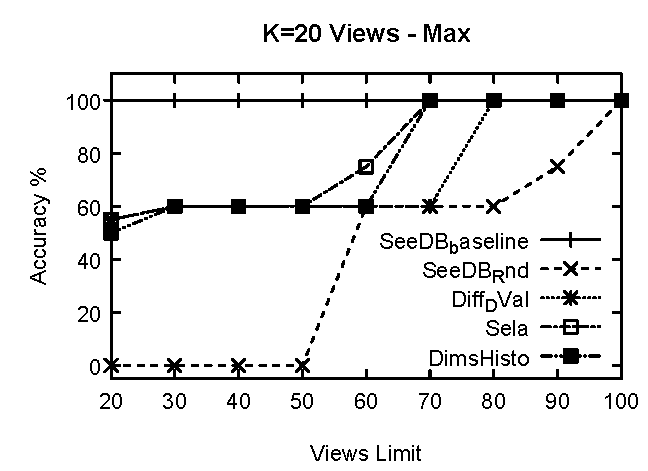
\includegraphics[width=\textwidth]{MaxA2.pdf}
    \caption{Max}
        \label{fig:MaxA2}%
  \end{subfigure}
  %
  \begin{subfigure}[b]{0.42\textwidth}
    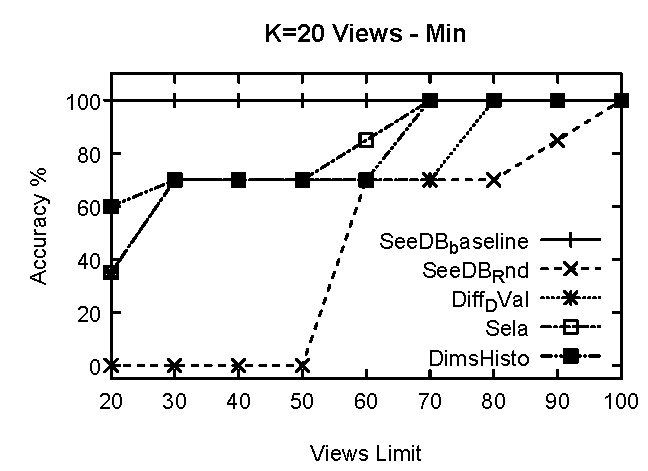
\includegraphics[width=\textwidth]{MinA2.pdf}
     \caption{Min}
        \label{fig:MinA2}
	% \caption{Accuracy on varying view space sizes for the Algorithms $Sela$ ,$Diff_DVal$, $DimsHisto$, and $SeeDB_Rnd$}
  \end{subfigure}
  \caption{Accuracy on varying view space sizes for the Algorithms $Sela$ ,$Diff_DVal$, $DimsHisto$, and $SeeDB_Rnd$}
\end{figure}
%\end{center}

%\begin{center}
  
\begin{figure}[h]
  \centering

  \begin{subfigure}[b]{0.42\textwidth}
    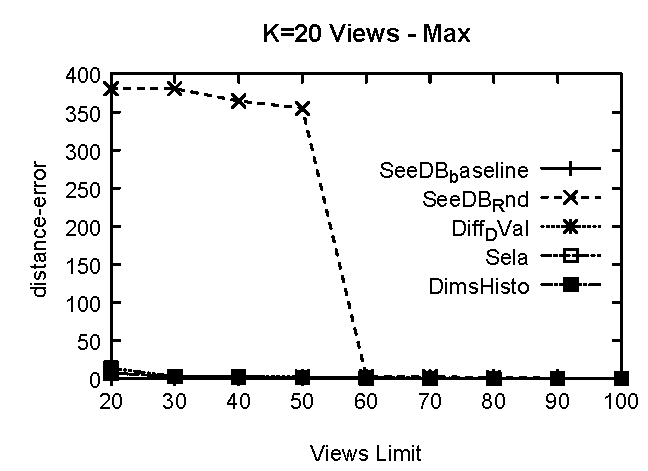
\includegraphics[width=\textwidth]{MaxD2.pdf}
    \caption{Max}
        \label{fig:MaxD2}%
  \end{subfigure}
  %
  \begin{subfigure}[b]{0.42\textwidth}
    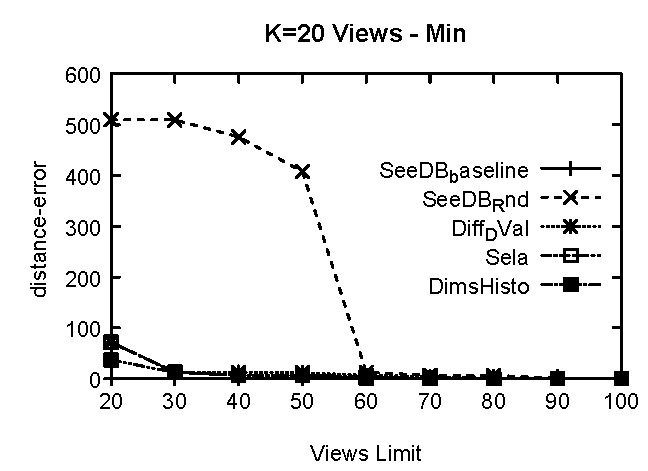
\includegraphics[width=\textwidth]{MinD2.pdf}
     \caption{Min}
        \label{fig:MinD2}
  \end{subfigure}
  
  \caption{Distance-error on varying view space sizes for the Algorithms $Sela$ ,$Diff_DVal$, $DimsHisto$, and $SeeDB_Rnd$}
\end{figure}

%\end{center}

In conclusion, the proposed techniques recommend high quality views in different views limits furthermore, the accuracy is increasing and it doesn't fluctuate along various views limits and similarly the distance-error is declining while increasing the number of explored views (views limit). In the worst cases, the accuracy and the distance-error remain fixed while increasing the number of explored views but they don't decrease. \\
%%%%%%%% Second Expr
\par In the following experiments, we vary $K$ — the number of visualizations
to recommend and fix the number of explored visualizations as \emph{Views Limit=70} and measure the accuracy, and error-distance for each of our
strategies along different aggregate functions. We pay special attention to k = 10 and 20 because empirically these k values are used most commonly.

In summary, $Sela$ and $DimsHisto$ algorithms both produce results with accuracy $100\%$ and zero distance-error when K=10 and 20 views for all aggregate functions as shown in figures \ref{fig:SumA1}, \ref{fig:AvgA1}, \ref{fig:CountA1}, \ref{fig:MaxA1}, and\ref{fig:MinA1} also algorithm $Diff_DVal$ scored accuracy $100\%$ in the first number of recommended views K=10 views. Although, $Diff_DVal$ obtains the same accuracy as $SeeDB_Rnd$ for all aggregate functions but the $Diff_DVal$ scores much better distance-error than $SeeDB_Rnd$ as shown in figures \ref{fig:SumD1}, \ref{fig:AvgD1}, \ref{fig:CountD1}, \ref{fig:MaxD1}, and\ref{fig:MinD1}. As discussed in the previous experiment, the $DimsHisto$ scores accuracy $100\%$ specifically when the aggregate functions \emph{Count} it is also succeeded to recommend views with $100\%$ and zero distance-error for aggregate functions \emph{Sum, Average, and Count} as shown in figures \ref{fig:SumA1}, \ref{fig:AvgA1}, and \ref{fig:CountA1}. In addition, we find that $Sela$ and $DimsHisto$ algorithms produce high quality views with $100\%$ accuracy and zero distance-error for \emph{Max} aggregate function , also they obtain $>75\%$ and $<0.2$ distance error for \emph{Min} aggregate function when k=70 (Views Limit ) as shown in \ref{fig:MaxD1} and \ref{fig:MinD1} receptively.

\begin{figure}[h]
  \begin{subfigure}[b]{0.32\textwidth}
    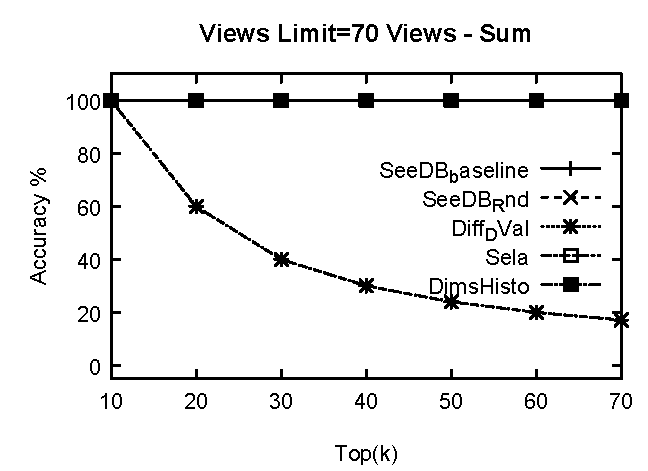
\includegraphics[width=\textwidth]{SumA1.pdf}
    \caption{Sum   }
        \label{fig:SumA1}%
  \end{subfigure}
  %
  \begin{subfigure}[b]{0.32\textwidth}
    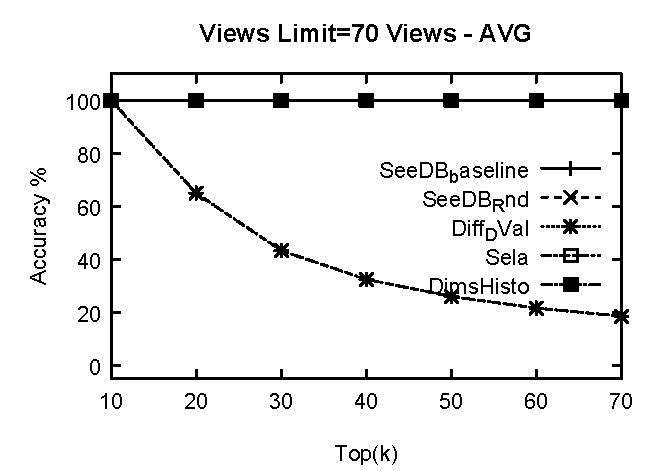
\includegraphics[width=\textwidth]{AvgA1.pdf}
     \caption{Average  }
        \label{fig:AvgA1}
  \end{subfigure}
  \begin{subfigure}[b]{0.32\textwidth}
    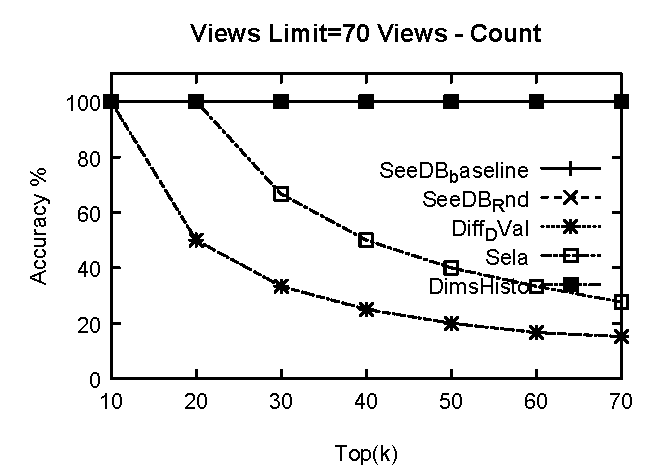
\includegraphics[width=\textwidth]{CountA1.pdf}
     \caption{count  }
        \label{fig:CountA1}
  \end{subfigure}
  \caption{Accuracy on varying view space sizes for the Algorithms $Sela$ ,$Diff_DVal$, $DimsHisto$, and $SeeDB_Rnd$}
\end{figure}

The following figures describe the distance error for the proposed algorithms, we find that although $Diff_DVal$ approach score the same accuracy produced by $SeeDB_Rnd$ strategy but it obtains very low distance error along all aggregate function compared with $SeeDB_Rnd$ strategy as shown in figures \ref{fig:SumD1}, \ref{fig:AvgD1}, \ref{fig:CountD1}, \ref{fig:MaxD1}, and\ref{fig:MinD1}. To Sum up, the proposed approaches boast the accuracy of the recommended views for the mostly common used K values. Moreover, the $Sela$ and $DimsHisto$ achieve better quality results than $Diff_DVal$  because they are capturing the data distribution in the dimension attributes by using selectivity ratios and frequency histograms.
 
\begin{figure}[h]
  \begin{subfigure}[b]{0.32\textwidth}
    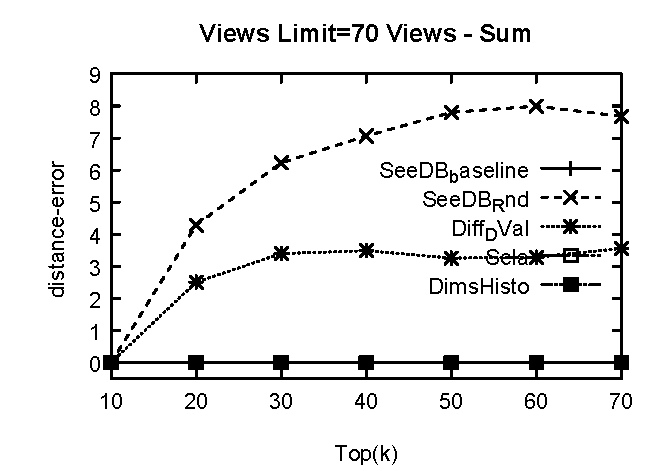
\includegraphics[width=\textwidth]{SumD1.pdf}
    \caption{Sum   }
        \label{fig:SumD1}%
  \end{subfigure}
  %
  \begin{subfigure}[b]{0.32\textwidth}
    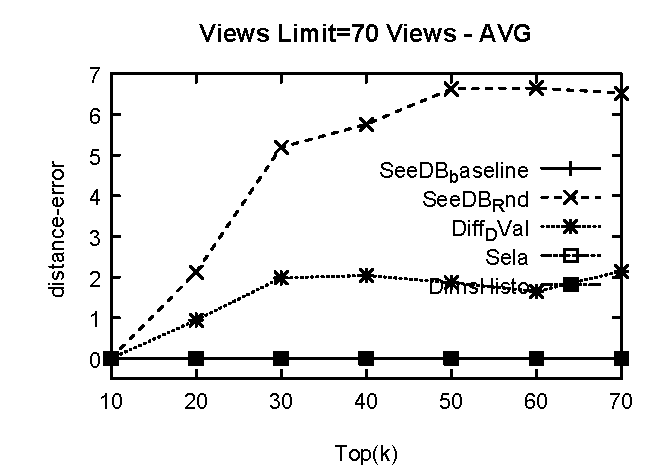
\includegraphics[width=\textwidth]{AvgD1.pdf}
     \caption{Average  }
        \label{fig:AvgD1}
  \end{subfigure}
  \begin{subfigure}[b]{0.32\textwidth}
    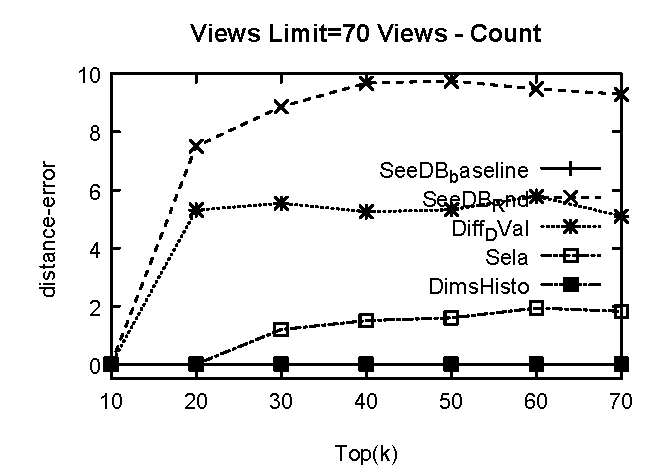
\includegraphics[width=\textwidth]{CountD1.pdf}
     \caption{count  }
        \label{fig:CountD1}
  \end{subfigure}
  \caption{Distance-error on varying k for the Algorithms $Sela$ ,$Diff_DVal$, $DimsHisto$, and $SeeDB_Rnd$}
\end{figure}


 % \begin{center}
    
  \begin{figure}[h]
  \centering
%\end{figure}
  \begin{subfigure}[b]{0.42\textwidth}
    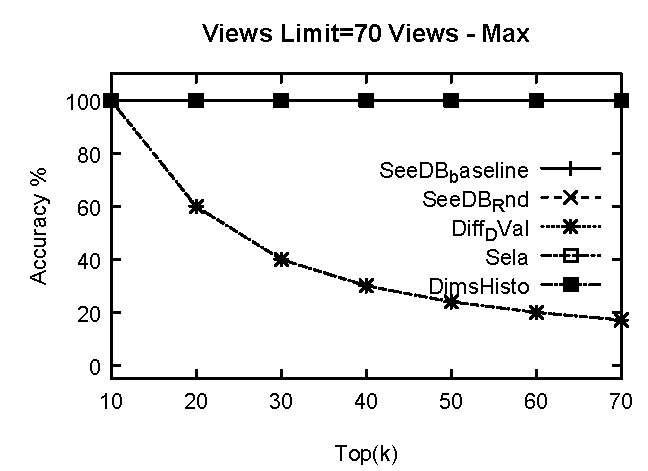
\includegraphics[width=\textwidth]{MaxA1.pdf}
    \caption{Max   }
        \label{fig:MaxA1}%
  \end{subfigure}
  %
  \begin{subfigure}[b]{0.42\textwidth}
    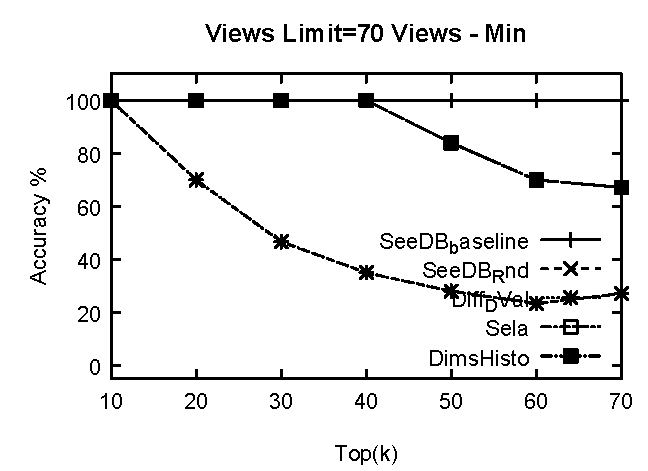
\includegraphics[width=\textwidth]{MinA1.pdf}
     \caption{Min  }
        \label{fig:MinA1}
  \end{subfigure}
  
  \caption{Accuracy on varying K for the Algorithms $Sela$ ,$Diff_DVal$, $DimsHisto$, and $SeeDB_Rnd$}
\end{figure}
%\end{center}

%\begin{center}
  
\begin{figure}[h]
  \centering
  \begin{subfigure}[b]{0.42\textwidth}
    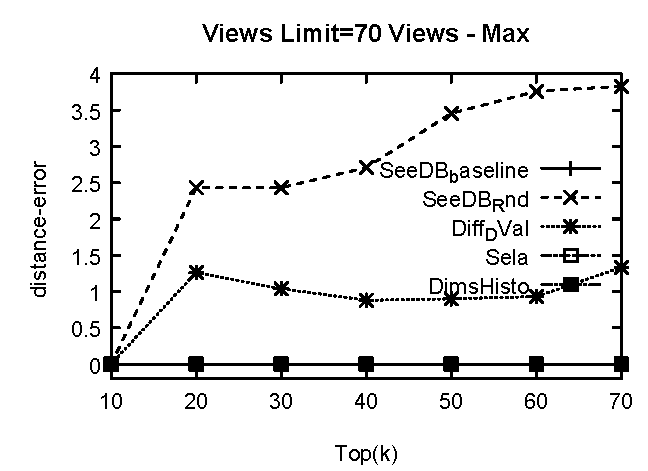
\includegraphics[width=\textwidth]{MaxD1.pdf}
    \caption{Max   }
        \label{fig:MaxD1}%
  \end{subfigure}
  %
  \begin{subfigure}[b]{0.42\textwidth}
    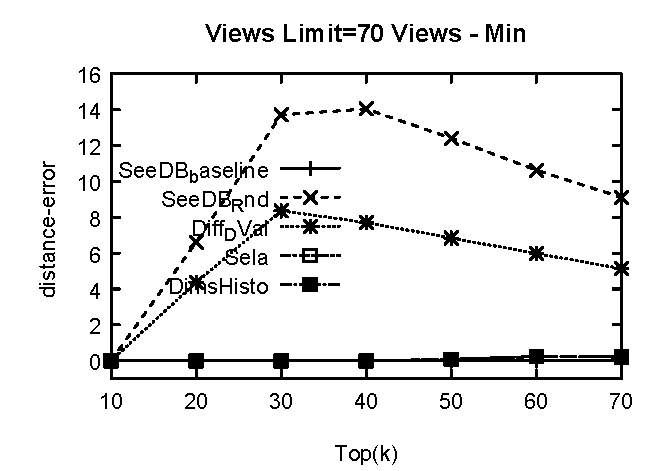
\includegraphics[width=\textwidth]{MinD1.pdf}
     \caption{Min  }
        \label{fig:MinD1}
  \end{subfigure}
  
  \caption{Distance-error on varying K for the Algorithms $Sela$ ,$Diff_DVal$, $DimsHisto$, and $SeeDB_Rnd$}
\end{figure} 

\subsection{Accuracy evaluation}
The dataset used is $GoCard$ data with size 4.4 M tuples contains 9 dimension attributes and 3 measures attributes with we run this experiment on SeeDB over \emph{All} aggregate functions \emph{Count, Sum, Average, Min, and Max} and total of all possible views in each dataset referred as a space size=$5 \times 9 \times 3=135$ views and 
the deviation metric is Earth Movers Distance (EMD). \\ %\mas{what is the input query(s)?} 
\footnotesize {$Q:$ Select * from gocard where alightingstop ='University of Queensland'} 

%\thefontsize 
\normalsize 
%\mas{use straight lines to connect points not curves}
%\mas{use the right accuracy metric}
we implement two baseline strategies. The SeeDB baseline strategy processes the entire data and does not discard any views ($SeeDB baseline$). It thus provides an upper bound on 
latency and accuracy and lower bound on error distance. The other baseline strategy we evaluate is the random strategy ($SeeDB_Rnd$) that returns a random set of k aggregate views as the result. This strategy gives a lower bound on accuracy and upper bound on error distance: for any technique to be useful, it must do significantly better than $SeeDB_Rnd$.
\\ In figure \ref{fig:fig1} shows the accuracy of the results produced by algorithms $Sela$ , $Diff_DVal$, $DimHisto$, and $SeeDB_Rnd$ to find a top $(K=25)$ views
 comparing with different view space sizes. As shown all proposed algorithms  $Sela$ and $Diff_DVal$ scored the same accuracy in the first 30 explored views however, algorithm $DimsHisto$ shows lower accuracy than $Sela$ and $Diff_DVal$ when the number of explored views is 45 because $DimHisto$ evaluates dimension attributes according to their frequencies and it's less descriptive to some aggregate functions such as Max and Min.  Thereafter, the proposed algorithms improve the accuracy to 100\% and keep accuracy stable without any fluctuation.
%\mas{so why it is not doing better when supposedly you proposed it to improve on the first one}
 In addition,  
all proposed algorithms maintain the accuracy of 
results while growing with the extension of the space size while other algorithm 
the accuracy remains stable. Finally, as shown  $SeeDB_Rnd$ is the lowest 
accuracy with different spaces except in the last two space limits. 

\begin{figure}[h]
  \centering
%\end{figure}
  \begin{subfigure}[b]{0.42\textwidth}
    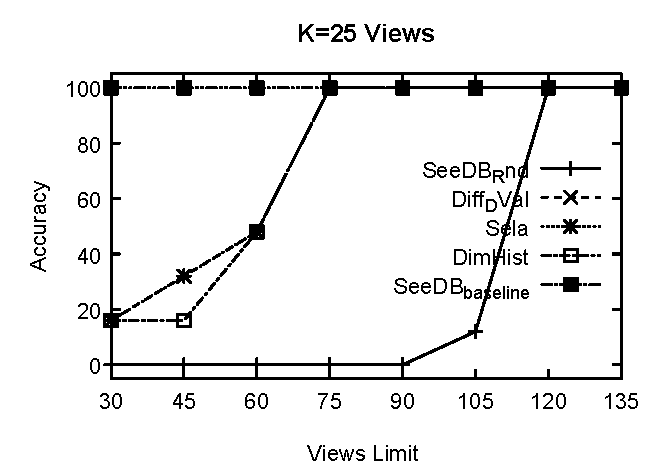
\includegraphics[width=\textwidth]{21.pdf}
    \caption{Accuracy}
        \label{fig:fig1}%
  \end{subfigure}
  %
  \begin{subfigure}[b]{0.42\textwidth}
    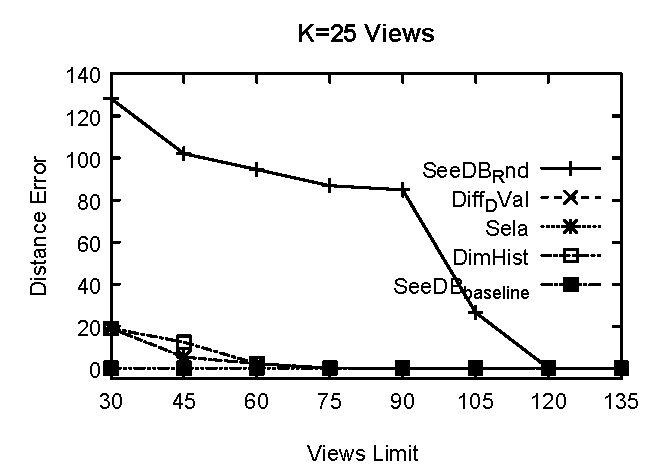
\includegraphics[width=\textwidth]{22.pdf}
     \caption{Error Distance}
        \label{fig:figa2}
  \end{subfigure}
  \caption{Results quality on varying view space sizes for the Algorithms $Sela$ ,$Diff_DVal$, $DimsHisto$, and $SeeDB_Rnd$}
\end{figure}

 %\begin{figure}[h]
%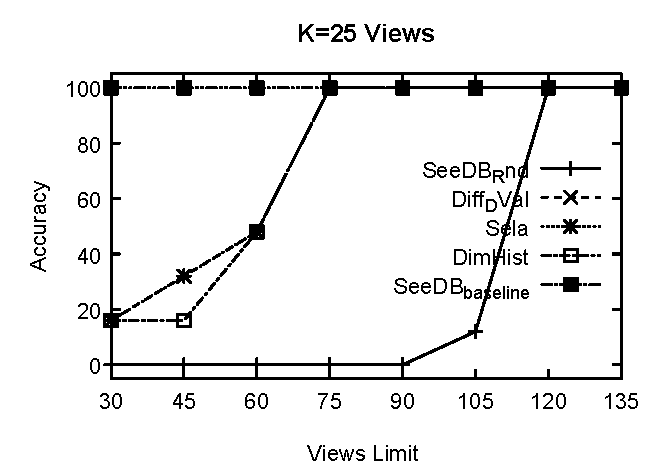
\includegraphics[width=\textwidth]{21.pdf}
%\caption{Accuracy compared with  the view space size for the Algorithms $Sela$ , $N-N'$, $DimHisto$, and $SeeDB_Rnd$}
%\label{fig:fig1}%
%\end{figure}

%\mas{use lines for all and only one y-axis}
In figure \ref{fig:figa2} shows the distance error of the results produced by
algorithms $Sela$ , $Diff_DVal$, and $DimsHisto$ to find a top $(K=25)$ views
 across different number of explored views denoted as 
space sizes as shown algorithms succeeded to minimize the distance error quickly near to $SeeDB Baseline$
specifically when the  
expansion of the space sizes. Although, algorithm $DimsHisto$ obtained lower 
accuracy than $Sela$ and $Diff_DVal$ as shown in figure \ref{fig:fig1} at view space 45, but the 
distance error at the same view space is low because $DimsHisto$ recommended 
different views with high utility distances to minimize the distance error.
%\mas{but supposedly the other two algorithms were two improve on it, but they did not - is that because they are poorly designed or what?}
Other algorithms succeeded to minimize the distance error quickly with 
expansion of the space sizes. 
$SeeDB_Rnd$ shows high distance error even if when the space size is large enough. 
%\begin{figure}[h]
%\includegraphics[width=\textwidth]{{22.pdf}}
%\caption{Error Distance according to the view space size for the Algorithms $Sela$ , $N-N'$, $DimHisto$, and $SeeDB_Rnd$}
%\label{fig:figa2}%
%\end{figure}

%\mas{That is a very shallow comment! You need to explain what happened and why?}
To sum up, the proposed algorithms evaluate the 
dimension attribute according to different priorities methods by recommending set of views 
which improve the quality of the view space limit R in terms of minimizing the distance error and 
enhancing the accuracy as shown in figures \ref{fig:fig1} and  \ref{fig:figa2}.
  
%  \begin{figure}[h]
%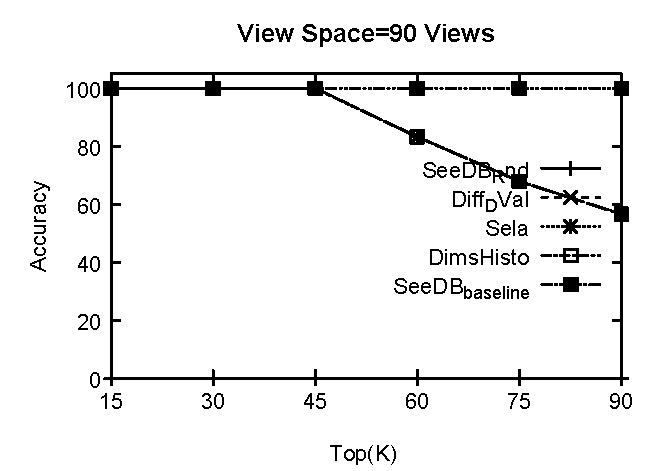
\includegraphics[width=\textwidth]{11.pdf}
%\caption{Accuracy compared with  top(K) views for the Algorithms $Sela$ , $N-N'$, $DimHisto$, and $SeeDB_Rnd$}
%\label{fig:fig3}%
%\end{figure}

\begin{figure}[h]
 \centering
%\end{figure}
  \begin{subfigure}[b]{0.42\textwidth}
    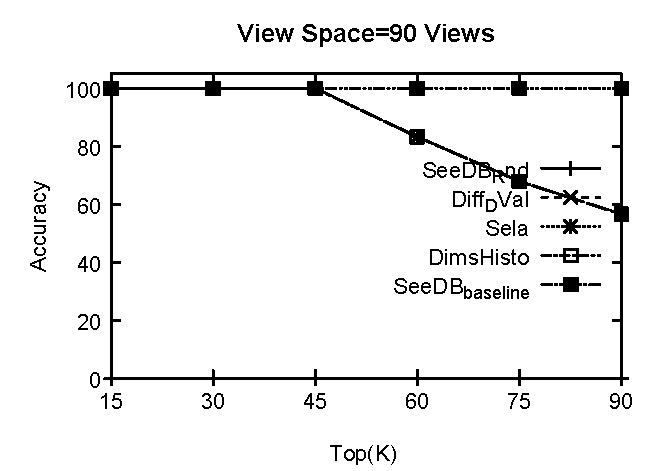
\includegraphics[width=\textwidth]{11.pdf}
    \caption{Accuracy  }
       \label{fig:fig3}
  \end{subfigure}
  %
  \begin{subfigure}[b]{0.42\textwidth}
    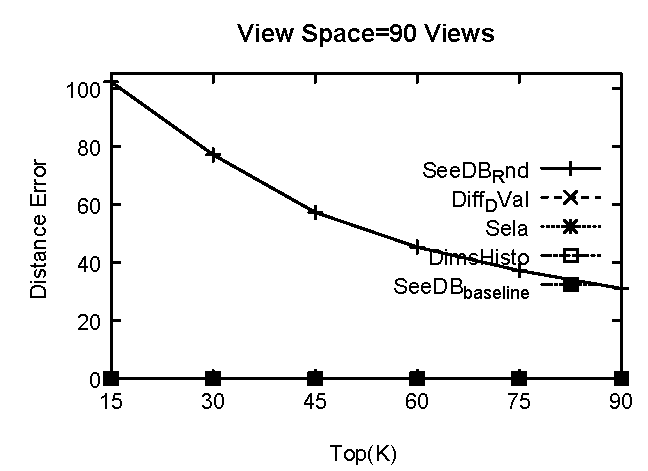
\includegraphics[width=\textwidth]{12.pdf}
     \caption{Error Distance  }
       \label{fig:fig4}%
  \end{subfigure}
  \caption{Results quality on varying top(K) views for the Algorithms $Sela$ , $Diff_DVal$, $DimHisto$, and $SeeDB_Rnd$}
\end{figure}

In figure \ref{fig:fig3} shows the accuracy of the 
algorithms $Sela$ , $Diff_DVal$, $DimsHisto$, and $SeeDB_Rnd$ in a fixed space size $R=90$ views
 comparing with different view 
space top(k) views as shown all algorithms scored 100\% accuracy in the first top 45 views 
which form half number of explored views.
We observe that the accuracy declines 
%\mas{why is that?!!} 
while increasing top(K) in a fixed space limit. 
This because wrong priortrizing of one dimension attribute than another will consequently affects on all 
recommended views that created from the wrong dimension attribute. However, the accuracy is above
50\% when k=90 (the entire view space limit) as shown in figure \ref{fig:fig3}. 
Furthermore, the analyst is usually interested in recommending a small number of 
visualisations e.g. k=25. 
%\begin{figure}[t]
%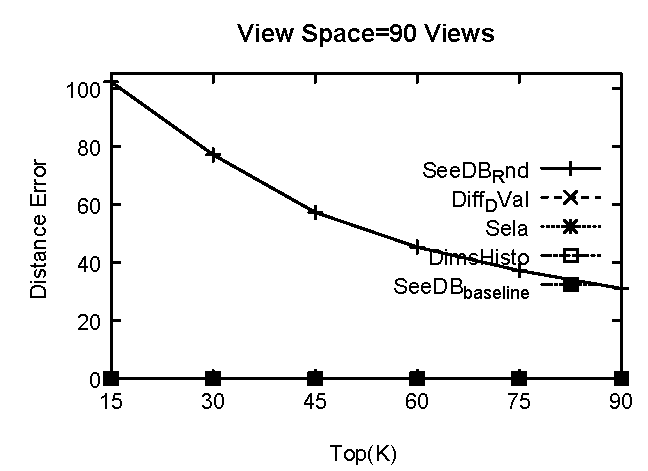
\includegraphics[width=\textwidth]{12.pdf}
%\caption{Error Distance compared with  the view space size for the Algorithms $Sela$ , $N-N'$, $DimHisto$, and $SeeDB_Rnd$}
%\label{fig:fig4}%
%\end{figure}

%\mas{again, what you proposed as better algorithms, performed worse than the basic one, why?!}
In figure \ref{fig:fig4} shows the distance error  of the 
algorithms $Sela$ , $Diff_DVal$, $DimHisto$, and $SeeDB_Rnd$ in a fixed space size $R=150$ views
 comparing with different Top(K) views 
 all algorithms have a very small distance error $\approx 0$ for Top(60) views
 however, $Diff_DVal$algorithm 
shows the smallest distance error across different K sizes. Both $Sela$  and $DimHisto$ 
report growing rise in the distance error with respect to Top(K) views required 
by the user in the certain view space size=90 views.\\

 In conclusion, the discussed algorithms $Sela$ ,$Diff_DVal$, $DimHisto$ show high 
 accuracy and low distance errors along different space sizes and 
 varying Top(K) as  illustrated previously however,
  these algorithms differentiate on the quality measures .For instance, 
 algorithm $Sela$ and $Diff_DVal$ 
 gain the highest accuracy than $DimHisto$ in the experiments as shown in
 figures  \ref{fig:fig1} and \ref{fig:fig3} but algorithm $Diff_DVal$  has the lowest error distance as shown in figures  \ref{fig:figa2} and \ref{fig:fig4}. 
 %
 \subsection{Efficiency evaluation}
  In this section, we evaluated the efficiency of the prioritizing algorithms in terms of the execution overhead added to 
	SeeDB (as automatic recommendation engine) by computing the costs of executing the proposed algorithms and gains of applying 
	the algorithms. Similarly, as the previous experiments, we measured the efficiency the algorithms 
	by running experiments to capture the overhead and the gains 
	along different $Top(K)$ and varying space limits compared with the actual execution of SeeDB baseline. 
 All the experiments were repeated 5 times and the measurements were averaged. We begin by presenting a summary of our experimental
findings and then dive into performance results for individual optimizations.

we compared the executions costs of the algorithms added to SeeDB with the original 
baseline of SeeDB to identify the improvements in the performance. As
shown in figure \ref{fig:fig33} shows the total SeeDB and algorithms execution 
times compared with the original SeeDB baseline. This figure shows the improvements
in the SeeDB performance with different space limits to find a top (K = 25) views. 
As shown the 
improvements in the performance by using the proposed algorithms 
are significant compared with the baseline furthermore, the execution costs increase linearly 
with the view space limit produced by algorithms. 
%\mas{what happens after 120? do the other two also exceed SeeDB?}
\begin{figure}
   \centering
%\end{figure}
  \begin{subfigure}[b]{0.42\textwidth}
    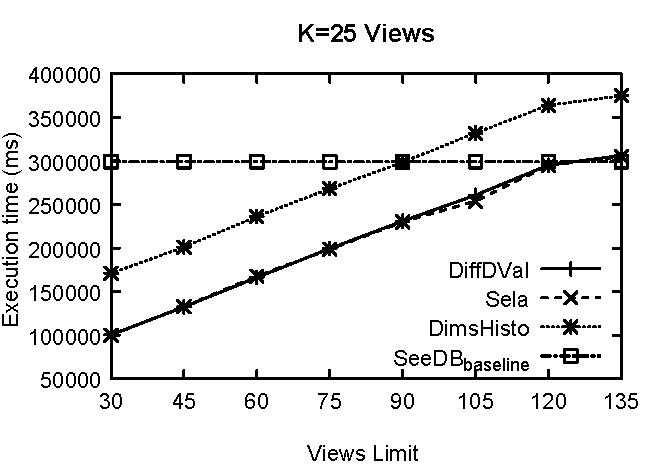
\includegraphics[width=\textwidth]{33.pdf}
    \caption{Execution times of algorithms across views limits}
    \label{fig:fig33}
  \end{subfigure}
  %
  \begin{subfigure}[b]{0.42\textwidth}
    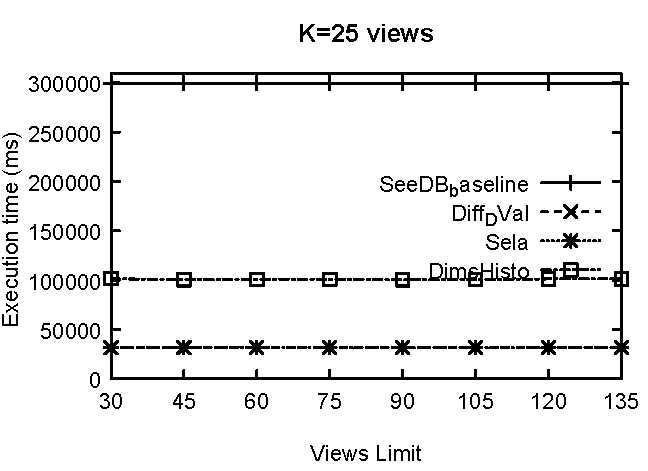
\includegraphics[width=\textwidth]{34.pdf}
    \caption{The overhead costs of proposed algorithms}
    \label{fig:fig34}
  \end{subfigure}
  \caption{Algorithms Performance on different space limits}
\end{figure}

%\mas{very confusing plot! what are the different components? and what are they stacked on top of each other?}
In Figure \ref{fig:fig34} illustrates the executions times of the 
algorithms $Sela$ , $Diff_DVal$ and $DimsHisto$ across different space limits 
however, this cost is considered as extra overhead should be added. As presented 
the executions times of the algorithms are almost stable along different space sizes 
because the algorithms evaluate a fixed set of dimension attributes every time. 
However, algorithm $DimsHisto$ is costly as it poses same number of queries to create histograms
then it computes the distance among those histograms.\\

\begin{figure}
   \centering
%\end{figure}
  \begin{subfigure}[b]{0.42\textwidth}
    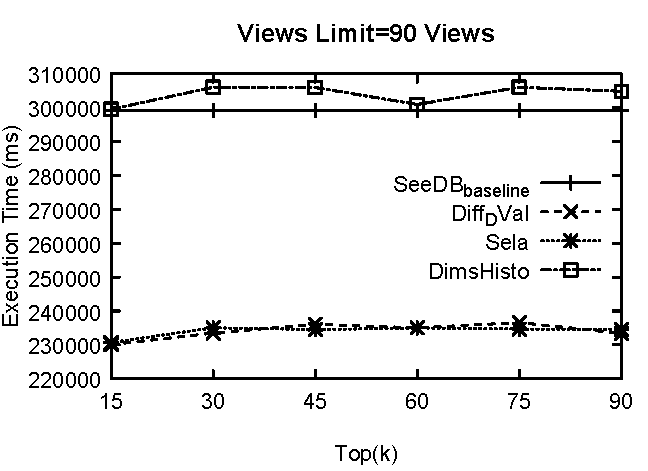
\includegraphics[width=\textwidth]{31.pdf}
    \caption{Total Execution time of the algorithms on fixed space limit}
    \label{fig:fig31a}
  \end{subfigure}
  %
  \begin{subfigure}[b]{0.42\textwidth}
    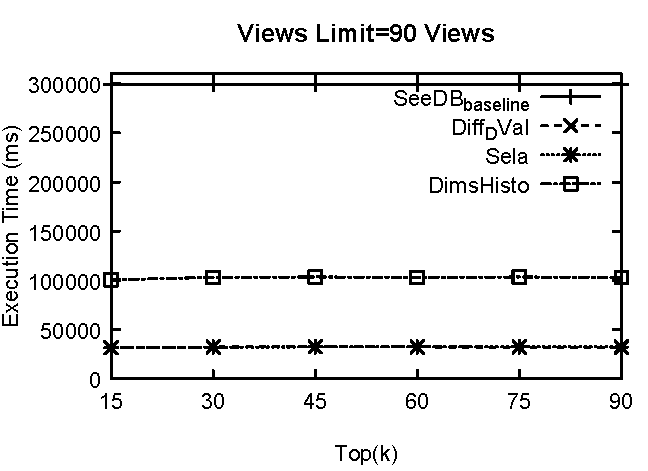
\includegraphics[width=\textwidth]{32.pdf}
    \caption{Overhead costs of the algorithms on fixed space limit}
    \label{fig:fig32}
  \end{subfigure}
  \caption{Algorithms Performance on varying $Top(k)$ views}
\end{figure}

The following figures discuss the efficiency of the proposed algorithms along different 
$Top(K)$ views in a certain space limit=90. As shown in figure 
\ref{fig:fig31a}, the proposed algorithms show improvements in the execution more 
than 40\% compared with the SeeDB baseline execution time. As discussed earlier, 
algorithm $DimsHisto$ shows the highest cost among algorithms $Sela$ and $Diff_DVal$. 
In other hand, figure \ref{fig:fig32} describes the execution costs of the algorithms separately. 
The running costs of algorithms are fixed while expanding $K$ the number of top deviated views 
because the algorithms run on a specified 
space limit.




 